
\chapter{Problem \& Background}

As discussed in the executive summary, the purpose of this project is to investigate and build a scaled down VTVL rocket which uses rotors and propellers to generate thrust for landing rather than a combustible fuel. The rotor arms and landing legs must be deployable during landing to accommodate a hypothetical launch scenario where the rocket was coming back to the ground and be guided to a landing pad.

One of the intended applications of this design is the NASA Student Launch Competition (NSL), which is an annual collegiate rocketry competition. The Northwestern Space Technology and Rocketry Society (NUSTARS) participates in this competition each year. Competition criteria change yearly; however, there are unvarying rules that follow national flight regulations. One important criterion prohibits the use of combustion fuel thrusters following initial ascent. This project will therefore be constrained following NSL’s competition rules so that NUSTARS can use this developed technology in the future. 

Our client, Professor Sridhar Krishnaswamy, was motivated to pursue this project based on the ongoing development by aerospace companies to create commercial and reusable rockets. In particular, the safe landing of aerospace vehicles in urban environments. Thus, another aim of this project is to investigate scaled down technologies that could theoretically aid in safely returning humans from extraterrestrial missions.

The scope of the project includes initial acceleration due to free fall, deployment of propulsion to slow down the vehicle, deployment of landing gear to land the vehicle upright, and controlled navigation to a desired landing zone. However, in our new new storyboard, we highlight the aspects of the project that we achieved, along with a potential step of hitting a hover, which we believe that we could accomplish quickly with the proper safety equipment. Hitting a hover would allow the rocket to behave in a manner similar to a quad copter, making the landing process easier. This storyboard is shown is figure \ref{fig:storyboard}.

\begin{figure}
    \centering
    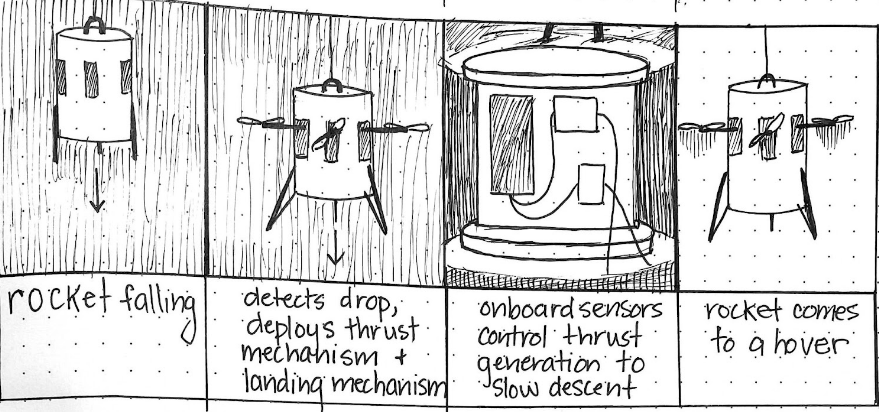
\includegraphics[width = 0.5\textwidth]{src/figs/Storyboard.png}
    \caption{New Updated Storyboard}
    \label{fig:storyboard}
\end{figure}

%MISSION STATEMENT
\clearpage
\section{Mission statement}
Our project seeks to develop a scaled rocket landing system capable of landing a rocket
vertically on a movable landing pad, while adhering to requirements set forth by NASA’s
Student Launch Competition, to broaden capabilities of rocket re-usability and missions.
